\section{Merge Sort}

Adotta l'approccio divide et impera, quindi:
\begin{itemize}
    \item divide: prende il problema originale e lo divide in problemi più piccoli.
    \item impera: ricorsivamente, risolve i sottoproblemi; se abbastanza piccolo, si risolve subito.
    \item combina: le soluzioni di $P_1$,...,$P_k$ si combinano in una soluzionedi $P$.
\end{itemize}

Quindi, mergesort adotta i seguenti passi:
\begin{itemize}
    \item dividere l'array in due parti
    \item ordina i sottoarray
    \item fonde i sottoarray ordinati
\end{itemize}

\begin{center}
    \begin{tabular}{c}
        \\ 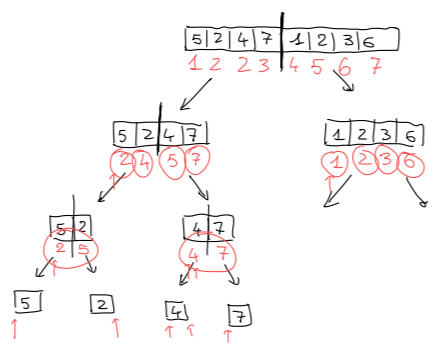
\includegraphics[width=0.6\textwidth]{image/MergeSortExample.png} \\ \\
    \end{tabular}
\end{center}

\newpage
\subsection{Pseudocodice}
\begin{mdframed}
\begin{lstlisting}[language=C]
MERGE-SORT(A,p,r)
1   if p < r
2       q = (p+r)/2
3       MERGE-SORT(A,p,q)
4       MERGE-SORT(A,q+1,r)
5       MERGE(A,p,q,r)
\end{lstlisting}
\end{mdframed}
\begin{mdframed}
\begin{lstlisting}[language=C]
MERGE(A,p,q,r)
1   n1 = q - p + 1
2   n2 = r - q
3   for i = 1 to n1
4       L[i] = A[p+i-1]
5   for j = 1 to n2
6       R[j] = A[q+j]
7   L[n1+1] = R[n2+1] = infinity
8   i = j = 1
9   for k = p to r
10      if L[i] <= R[j]
11          A[k] = L[i]
12          i = i + 1
13      else // L[i] > R[j]
14          A[k] = R[j]
15          j = j + 1
\end{lstlisting}
\end{mdframed}

\subsection{Complessità}
$A[p, ..., k-1]$ contiene $L[1, ..., i-1]$ e $R[i, ..., j-1]$
$A[p, ..., k-1] \leq L[1, ..., n_1-1]$ e $R[i, ..., n_2-1]$ è ordinato

\paragraph{Inizializzazione:} $k=p$ e $A[p, ..., k-1] = A[p, p-1]$
\paragraph{Mantenimento:} Divisione in due metà progressive dell'array
\paragraph{Conclusione:} $K = r+1$ e $A[p, ..., r]$ è ordinato e contiene i più  piccoli elementi $L[1, ..., n_1+1]$ e $R[1, ..., n_2+1]$

La dimostrazione del perchésia corretto viene fatta per induzione: se vale per il primo elemento, vale per tutti i casi successivi.

\newpage